\documentclass[12pt,letterpaper]{article}
\usepackage{fullpage}
\usepackage[top=2cm, bottom=4cm, left=2cm, right=2cm]{geometry}
\usepackage{amsmath,amsthm,amsfonts,amssymb,amscd}
\usepackage{lastpage}
\usepackage{enumerate}
\usepackage{fancyhdr}
\usepackage{mathrsfs}
\usepackage{xcolor}
\usepackage{graphicx}
\usepackage{listings}
\usepackage{hyperref}
\usepackage{siunitx} % Formats the units and values
\usepackage{appendix}
\usepackage{caption}
\usepackage{subcaption}
\usepackage{multicol}
\usepackage{wrapfig}
\usepackage{esint}
\usepackage[utf8]{inputenc}
\usepackage[T1]{fontenc}
\usepackage[inline]{enumitem} %allows inline itemize or enumerate
\usepackage{pdfpages}
\usepackage{booktabs} % For \toprule, \midrule and \bottomrule
\usepackage{pgfplotstable} % Generates table from .csv
\pgfplotsset{compat=1.16}
% Setup siunitx:
 \sisetup{
   round-mode          = places, % Rounds numbers
   round-precision     = 2, % to 2 places
 }


\hypersetup{%
  colorlinks=true,
  linkcolor=blue,
  linkbordercolor={0 0 1}
}
 
\renewcommand\lstlistingname{Algorithm}
\renewcommand\lstlistlistingname{Algorithms}
\def\lstlistingautorefname{Alg.}

\lstdefinestyle{Python}{
    language        = Python,
    frame           = lines, 
    basicstyle      = \tiny,
    keywordstyle    = \color{blue},
    stringstyle     = \color{green},
    commentstyle    = \color{orange}\ttfamily
}

\setlength{\parindent}{0.0in}
\setlength{\parskip}{0.1in}
\setlength{\tabcolsep}{6pt}

%Astronomical units
\DeclareSIUnit \parsec  {pc}
\DeclareSIUnit \year    {yr}

% Edit these as appropriate
% \newcommand\course{ASTRO 732}
% \newcommand\coursename{Computational Methods for Astrophysics}
\newcommand\course{ASTRO 645}
\newcommand\coursename{Astrophysical Dynamics}
\newcommand\hwnumber{5}
\newcommand\myname{Sandra Bustamante}  
%allows to number the last equation of align.
\newcommand\numberthis{\addtocounter{equation}{1}\tag{\theequation}}

\pagestyle{fancyplain}
\headheight 35pt
\lhead{\course \\ Homework \hwnumber}
\chead{\textbf{\Large Liouville and Boltzmann}}
%\rhead{\myname \\ Due October 29, 2019}
\rhead{\myname}
\lfoot{}
\cfoot{\coursename}
\rfoot{\small\thepage}
\headsep 1.5em

%redefines subsections to be letters instead of numbers so 1.a normal way is 1.1
% \arabic (1, 2, 3, ...)
% \alph (a, b, c, ...)
% \Alph (A, B, C, ...)
% \roman (i, ii, iii, ...)
% \Roman (I, II, III, ...)
\renewcommand\thesubsection{\thesection.\alph{subsection}}

%%%%%%%%%%%%%%%%%%%%%%%%%%%%%%%%%%%%%%%%%%%%%%%%%%%%%%%%%%%%%%%
%=====================BEGIN DOCUMENT===========================
%%%%%%%%%%%%%%%%%%%%%%%%%%%%%%%%%%%%%%%%%%%%%%%%%%%%%%%%%%%%%%%

\begin{document}
\twocolumn
\lstset{style=Python}

% textwidth is \the\textwidth \\
% column width is \the\columnwidth \\
% textheight is \the\textheight

\section{Collisionless Boltzmann \\Equation}

% Show that in a frame that rotates with constant angular velocity $\mathbf{\Omega}$,
% with $\nabla\mathbf{\Phi}_{eff}\equiv\mathbf{\Phi}-\frac{1}{2}|\mathbf{\Omega}\times\mathbf{x}|^2$, the collisionless Boltzmann equation can
% be written:
% \begin{equation}
%     \frac{\partial f}{\partial t}+\mathbf{v}\cdot\nabla f - \left[2(\mathbf{\Omega}\times\mathbf{v})+\nabla\mathbf{\Phi}_{eff}\right]\cdot\frac{\partial f}{\partial \mathbf{v}}=0
% \end{equation}
% [Hint: This is B\&T, Problem 4.1 on page 387.]

The continuity equation is
\begin{equation}
    \frac{\partial f}{\partial t} + \frac{\partial}{\partial w}\cdot (f\Dot{w})=0
\end{equation}
where we can consider $w=(p,q)$ as any arbitrary system of canonical coordinates \cite{BT2008} and $\Dot{w}\mathrm{is}(\Dot{p},\Dot{q})$. 
 
In a rotating frame, the canonical coordinates are $w=(x,v)$ and $\Dot{w}=(\Dot{x},\Dot{v})$ so the continuity equation is given by
\begin{align*}
    &\frac{\partial f}{\partial t} + \frac{\partial}{\partial \mathbf{w}}\cdot (f\Dot{\mathbf{w}})=0\\
    &\frac{\partial f}{\partial t} + \frac{\partial}{\partial \mathbf{x}}\cdot (f\Dot{\mathbf{x}})+ \frac{\partial}{\partial \mathbf{v}}\cdot (f\Dot{\mathbf{v}})=0\\
    &\frac{\partial f}{\partial t} + \frac{\partial f}{\partial \mathbf{x}}\cdot \Dot{\mathbf{x}} +\frac{\partial \dot{\mathbf{x}}}{\partial \mathbf{x}}\cdot f + \frac{\partial f}{\partial \mathbf{v}}\cdot \Dot{\mathbf{v}} + \frac{\partial \Dot{\mathbf{v}}}{\partial \mathbf{v}}\cdot f=0\\
    &\frac{\partial f}{\partial t} + \nabla f\cdot\Dot{\mathbf{x}} + \frac{\partial f}{\partial \mathbf{v}}\cdot \Dot{\mathbf{v}}=0.\numberthis{\label{eq:cont}}
\end{align*}
where 
\begin{align*}
    \mathbf{v}&=\dot{\mathbf{x}}\\
    \dot{\mathbf{v}}&=\Ddot{\mathbf{x}}=-\nabla\mathbf{\Phi} - 2\mathbf{\Omega}\times\dot{\mathbf{x}}-\mathbf{\Omega}\times(\mathbf{\Omega}\times\mathbf{x})\\
    &= -\nabla\mathbf{\Phi}_{eff} - 2\mathbf{\Omega}\times\dot{\mathbf{v}}
\end{align*}

Substituting the last equations into the continuity equation \ref{eq:cont} and  we get
\begin{align*}
    &\frac{\partial f}{\partial t} + \nabla f\cdot \mathbf{v} + \frac{\partial f}{\partial \mathbf{v}}\cdot (-\nabla\Phi_{eff} - 2\mathbf{\Omega}\times\dot{\mathbf{x}}) =0\\
    &\frac{\partial f}{\partial t}+\mathbf{v}\cdot\nabla f - \left(2\mathbf{\Omega}\times\mathbf{v}+\nabla\mathbf{\Phi}_{eff}\right)\cdot\frac{\partial f}{\partial \mathbf{v}}=0
\end{align*}




% % %\include{name} %name without extension. insert in new page
\newpage %continues on next column
%\clearpage %continues on next page

\section{Liouville equation and the pendulum}

Consider the pendulum of length l and mass m in a gravitational field
g. The kinetic energy and potential energy are
\begin{equation}
    T=\frac{1}{2}ml^2\dot{\theta}^2
\end{equation}
and 
\begin{equation}
    V=mgl(1-\cos\theta)
\end{equation}

\subsection{}
%Derive the Hamiltonian and write down Hamilton’s equations.
Starting from the Lagrangian, 
\begin{equation*}
    \mathcal{L}(\theta,\dot{\theta},t)\equiv T-V = \frac{1}{2}ml^2\dot{\theta}^2 - mgl(1 - \cos\theta),
\end{equation*}
we can find the generalized momentum by
\begin{align*}
    p\equiv\frac{\partial\mathcal{L}}{\partial\dot{q}}=ml^2\dot{\theta}.
\end{align*}
Then the Hamiltonian is
\begin{align*}
    \mathcal{H}&\equiv T+V\\
    \mathcal{H}&=\frac{1}{2}ml^2\dot{\theta}^2+mgl(1-\cos\theta)\\
    \mathcal{H}&=\frac{1}{2}\frac{p^2}{ml^2}+mgl(1-\cos\theta).
\end{align*}

Hamilton's equations are:
\begin{align*}
    \dot{p}&\equiv-\frac{\partial\mathcal{H}}{\partial\theta}=-mgl\sin\theta\\
    \dot{q}&\equiv\frac{\partial\mathcal{H}}{\partial p}=\frac{p}{ml^2}=\dot{\theta}
\end{align*}

\subsection{}
%Transform these equations to a non-dimensional set of variables $(q,p)\to(z_1,z_2)$ such that $\tau=\omega t$ where $\omega^2=g/l$ and the dimensionless energy is:
% \begin{equation}
%     \varepsilon\equiv\frac{E}{mgl}=\frac{1}{2}z_2^2+(1-\cos z_1)
% \end{equation}
% Show that $\tau_0=2\pi/\omega$ is the period of small oscillations  for this system.
From the dimensionless energy $\varepsilon=E/mgl$ 
\begin{align*}
    \varepsilon&=\frac{1}{mgl}\left[\frac{1}{2}ml^2\dot{\theta}^2+mgl(1-\cos\theta)\right]\\
    &=\frac{1}{2}\frac{l}{g}\dot{\theta} + (1-\cos\theta),
\end{align*}
we can find the dimensionless variables as
\begin{align*}
    z_1\equiv\theta\\
    z_2\equiv\frac{l}{g}\dot{\theta}=\frac{\dot{\theta}}{\omega^2}
\end{align*}
where $\omega^2=g/l$.

Knowing that the equation of motion for this system is 
\begin{equation*}
    \Ddot{\theta}=-\frac{g}{l}\sin\theta
    \label{eq:pendEqMotion}
\end{equation*}
we can find that the solution for this differential equation in the small angle approximation will be given by
\begin{equation*}
\frac{dz_2}{d\tau}=\frac{d}{dt}
\frac{\Ddot{\theta}}{\omega^2}=    
\end{equation*}


then, we can show that
$\tau_0=2\pi/\omega$.

\subsection{}
%Sketch the phase portrait in these units, paying special attention to
% the three domains: 1) $\varepsilon<2$, the oscillation  or libration regime; 2) $\varepsilon>2$, the rotation regime 3)$\varepsilon=2$, the critical infinite period, the separatrix.

\begin{figure}
    \centering
    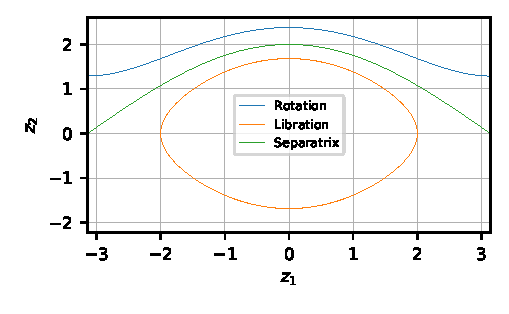
\includegraphics{CodeAndFigures/PendulumPhaseSpace.pdf}
    \caption{Phase Space of a pendulum in rotation, libration and separatrix.}
    \label{fig:pendPhaseSpace}
\end{figure}
We can integrate the pendulum's equation of motion \ref{eq:pendEqMotion} using a 4th order Runge-Kutta and the initial conditions listed in table



\begin{enumerate}
\item Consider a disk-like domain of initial configurations $U_s$ enclosed
within the circle centered at $(q,p)=(z_1,z_2)=(0,1)$ with radius
of $1/2$ in these units. See Fig. 1 for a plot of these initial conditions. Compute the evolution of the disk from $\tau=0$ to each of $\tau=0.25\tau_0,0.5\tau_0,\mathrm{and}\tau_0$.
Remarks:
    \begin{itemize}
    \item Argue that it is sufficient to compute the trajectories on the
    circle at edge of the disk. In other words, a point on the inside
    of the disk can not pass through a boundary point.
    \item You may solve this any way you like. E.g. there is an analytic
    solution in terms of elliptic integrals. But I recommend an
    numerical solution, using your RK4 routine to solve the equations of motion for say 32 points equally spaced around the
    circle at the perimeter of $U_s$ at $\tau = 0$.
    \item For insight consider this problem in the small angle limit. In
    this limit, the solution is analytic. If you have any worries
    about your solution, make sure it agrees with the small angle limit.
    \end{itemize}
\item Repeat the experiment but now with the circle centered at $(q,p)=(0,1.5)$ Note: some points will be on or near the seperatrix. Compute the evolution of the disk for $\tau=0,0.2\tau_0,0.4\tau_0,\mathrm{and}0.75\tau_0$.[NB: the “evolution” at t = 0 is the initial condition, of course.]
\item Repeat the experiment but now with the circle centered at  $(q,p)=(0,2)$. Compute the evolution at times $\tau=0,0.1\tau_0,0.25\tau_0,\mathrm{and}0.5\tau_0$ 
\item For each of the three experiment with different disk centers, make
a plot the disk at each of these times in the $(q,p)$ plane (e.g.
a phase portrait). Interpret the results. Is Liouville’s theorem obeyed?
\end{enumerate}




% A symplectic integrator is an integrator that conserve phase-space volume and Poincar\' e invariants \cite{BinneyT_}

% Leapfrog integrator is a second order method that integrates ordinary differential equations. It updates the position and velocity at interleaved times. The algorithm is being implemented is of the sequence drift-kick-drift. A drift is when the position $\Vec{q}$ changes but not the momentum $\Vec{p}$ and a kick is the inverse, momentum changes but not the position. The algorithm is
% \begin{align*}
%     \Vec{q}_{1/2}&=\Vec{q}_0+\frac{1}{2}h\Vec{p_0}\\
%     \Vec{p}&=\Vec{p}_0 + h F(\Vec{q}_{1/2})\\
%     \Vec{q}&=\Vec{q}_0 + \frac{1}{2}h\Vec{p}
% \end{align*}
% where $F(\Vec{q}_{1/2})$

% We can test the leapfrog algorithm using the pendulum. 
% The equation of motion of the pendulum is given by
% \begin{equation}
%     \Ddot{\theta}=-\sin\theta.
% \end{equation}

% We can determine 3 scenarios:
% \begin{itemize}
%     \item Rotation \\
%     It is when the total energy given by
%     \begin{equation}
%     E=\frac{1}{2}\Dot{\theta}^2+\left(1+\cos\theta\right)
%     \end{equation}
%     is bigger than the critical energy. The critical energy is given by the energy evaluated in equilibrium. For this case, is 2. If thinking of a physical pendulum, we can make the pendulum go to rotation when we start it with an added velocity.
%     \item Libration \\
%     It is when the total energy is smaller than the critical energy. This is where the pendulum oscillates with small amplitudes. We can achieve this when we drop the pendulum at an angle close to equilibrium.
%     \item Equilibrium \\
%     It is where the pendulum stays in equilibrium. This can happen when the pendulum is straight down or straight up. When it is straight up it is called an unstable equilibrium since a very small force can take it out of that state. 
% \end{itemize}
% These 3 scenarios can be created by using the initial conditions listed in table \ref{tab:PendulumIV}.

% \begin{table}
%     \centering
% \input{CodeAndFigures/PendulumData.tex}
%     \caption{Initial conditions use for the integration of the pendulum for the case of rotation, libration and near the unstable equilibrium.}
%     \label{tab:PendulumIV}
% \end{table}

% % \begin{figure}
% %     \centering
% %     \includegraphics{CodeAndFigures/PendulumXYPlot.pdf}
% %     \caption{Plot showing the movement of the pendulum for each scenario.}
% %     \label{fig:pendulumOrbitPlot}
% % \end{figure}

% % Figure \ref{fig:pendulumOrbitPlot} shows the trajectory of the pendulum for each scenario. 

% \begin{figure*}[ht!]
%     \centering
%     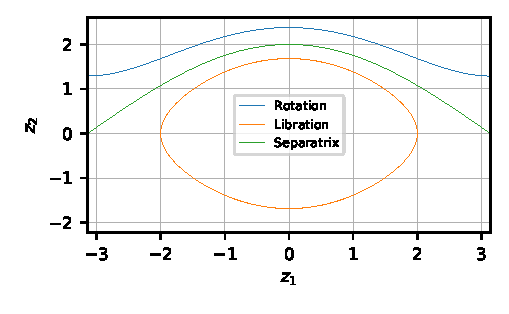
\includegraphics{CodeAndFigures/PendulumPhaseSpace.pdf}
%     \caption{Plot of the phase space for each scenario using Leapfrog and 4th order Runge-Kutta (RK4).}
%     \label{fig:pendulumPhaseSpace}
% \end{figure*}

% Figure \ref{fig:pendulumPhaseSpace} shows the phase space of each scenario using leapfrog integration and 4th order Runge-Kutta. When the pendulum is in libration it forms concentric circles near the stable equilibrium while in rotation it forms curve lines above the critical energy. When the pendulum is near the unstable equilibrium it forms an oblate shape where it almost touches the unstable equilibrium point. 
% % (b) Demonstrate that the leapfrog integrator is second-order accurate
% % in the sense that errors in $\mathbf{q}$ and $\mathbf{p}$ after a time step $h$ are $O(h^3)$.

% \begin{figure*}[ht!]
%     \centering
%     \includegraphics[width=\textwidth]{CodeAndFigures/PendulumErrorvsStepsize.pdf}
%     \caption{Plots of errors at different time steps $h$ for each scenario: rotation, libration and near unstable equilibrium.}
%     \label{fig:pendulumErrors}
% \end{figure*}

% Figure \ref{fig:pendulumErrors} shows the errors in position and velocity of leapfrog with different time steps. The error was calculated by subtracting the final value of position at a time step minus the final value at the previous time step, where the time step at each iteration gets halved. 

% Note that at smaller time steps the error $\mathcal{O}(h^3)$ ie. the error is of second order represented by the line $h^2$. At larger time steps, equivalently the time steps is almost the same as the orbit period so it will suffer from variation equivalent to under sampling a signal in digital systems.

% % (c) Compute the energy conservation for the trajectories in each regime
% % over about 10,000 orbital periods. Compare the energy conservation for RK4 and leapfrog.
% \begin{figure*}[ht!]
%     \centering
%     \includegraphics{CodeAndFigures/PendulumRK4vsLeapfrog.pdf}
%     \caption{Plots comparing the calculated total energy through time using leapfrog integrator and RK4 integrator for each scenario of the pendulum system.}
%     \label{fig:pendulumEnergy}
% \end{figure*}

% Figure \ref{fig:pendulumEnergy} shows the total energy of the pendulum of the 3 scenarios over 10,000 orbits. It shows that when using the leapfrog integrator, the energy has small variations but remains constant in a small range through time, in other words, energy is being conserved, while the total energy using RK4 shows a drift, energy is not conserved. This is one of the advantages of leapfrog over RK4 for dynamical systems where the energy needs to be conserved.

\newpage

% \input{problem3.tex}
% \newpage

% \input{problem4.tex}
% \newpage

% \input{problem5.tex}
% \newpage

% \input{problem6.tex}
%\newpage

%%%%%%%%%%%%%%%%%%%%%%%%%%%%%%%%%%%%%%%%%%%%%%%%%%%%%%%%%%%%%%%
%=====================Add Bibliography=========================
%%%%%%%%%%%%%%%%%%%%%%%%%%%%%%%%%%%%%%%%%%%%%%%%%%%%%%%%%%%%%%%

\bibliographystyle{plain} % We choose the "plain" reference style
%plain style sorts the reference list by alphabetical order of the first author’s last name.
\bibliography{references} % Entries are in the "refs.bib" file

\clearpage

%%%%%%%%%%%%%%%%%%%%%%%%%%%%%%%%%%%%%%%%%%%%%%%%%%%%%%%%%%%%%%%
%=====================Appendix=================================
%%%%%%%%%%%%%%%%%%%%%%%%%%%%%%%%%%%%%%%%%%%%%%%%%%%%%%%%%%%%%%%
 \appendix

\section[]{Python code} 
\lstset{caption={Astro645HW05p2.py}, style=Python}
%\label{sec:CodeHw04p1}
%\lstset{label={Astro732Hw04P1.py}}
\lstinputlisting[language=Python]{CodeAndFigures/Astro645HW05p2.py}

\newpage

%\section[]{Python code Problem 3} 
\lstset{caption={SetupPlots.py}, style=Python}
\lstinputlisting[language=Python]{CodeAndFigures/SetupPlots.py}

\newpage

%\section[]{Python code Problem 4} 
\lstset{caption={NumericIntegrations.py}, style=Python}
\lstinputlisting[language=Python]{CodeAndFigures/NumericIntegrations.py}

% \newpage

% %\section[]{Python code Problem 5} 
% \lstset{caption={Astro645HW04p5.py}, style=Python}
% \lstinputlisting[language=Python]{CodeAndFigures/Astro645HW04p5.py}


\end{document}